\subsection{Hybrid approach}

There are two variant of hybrid methods; the first is hybrid on triangle pairs and the second is hybrid on triangle pairs. Both variants are developed to exploit both the robustness of brute force and the arithmetic intensity of the penalty method.

show penalty histogram here


\begin{figure}[!h]
\centering
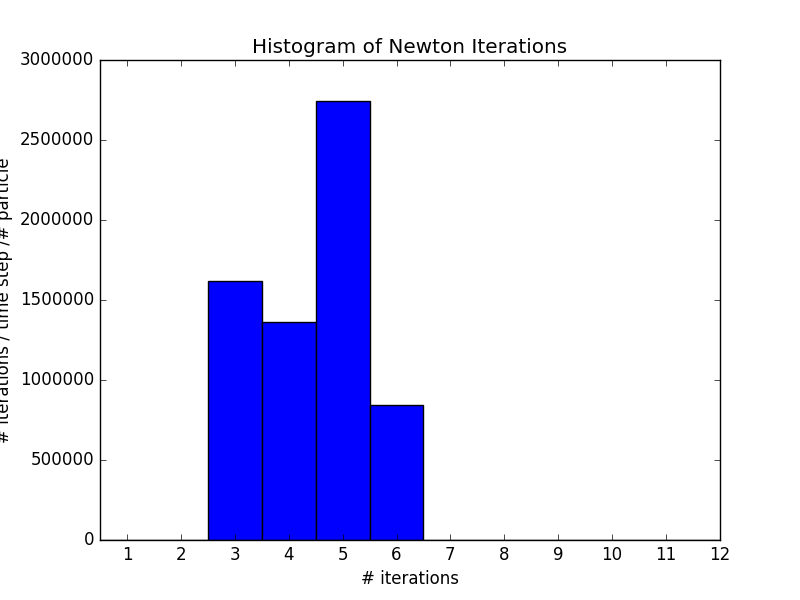
\includegraphics[width=1\textwidth]{experiments/random/newton_histogram} \protect\caption{\label{fig17}Newton solver histogram of number of iterations for convergence.}
\end{figure} 

The hybrid on triangle pairs is splitting the workload of detecting the contact points between two particles by being hybrid on each triangle pair. Per triangle pair the penalty solver is run first and per triangle pair if the solution is not within a user specified tolerance, we fall back to brute force to solve the problem robustly.  

ALGORITHM HYBRID-ON-TRIANGLES GOES HERE

\begin{algorithm}
 \caption{Hybrid on triangle batches} \label{algorithm:bf}
 \begin{algorithmic}[1]
	
	\State $FOR i = 0 to n/batchSize$

		\State $batch[i] to batchSize$		
					
			\State $penalty()$

		\State $ENDFOR$

		\State $IF batchError[i] > epsilon$

			\State $FOR batch[i] to batchSize$
	
				\State $bruteForce()$

			\State $ENDFOR$
	
		\State $ENDIF$
	
	\State $ENDFOR$
	
 \end{algorithmic}
\end{algorithm} 


ALGORITHM HYBRID-ON-BATCHES GOES HERE

\begin{algorithm}
 \caption{Hybrid on triangle pairs} \label{algorithm:bf}
 \begin{algorithmic}[1]
	
	\State $FOR i = 0 to n$
	
		\State $penalty()$

		\State $IF triangleError[i] > epsilon$

				\State $bruteForce()$
	
		\State $ENDIF$
	
	\State $ENDFOR$
	
 \end{algorithmic}
\end{algorithm} 


The other variant is the hybrid on batches where it is hybrid per triangle batches instead of a pair. This method is checking the error less frequently than the previous variant. As in the hybrid-on-triangle-pairs variant; we run penalty on one batch of triangles and then fall back to brute for the whole batch if the error tolerance is not satisfied. The batch size can be set by the user but for our applications/setup we set it to be the number of triangles of our non-spherical particles (mesh size of 60~ triangles).    


hybrid vectorization
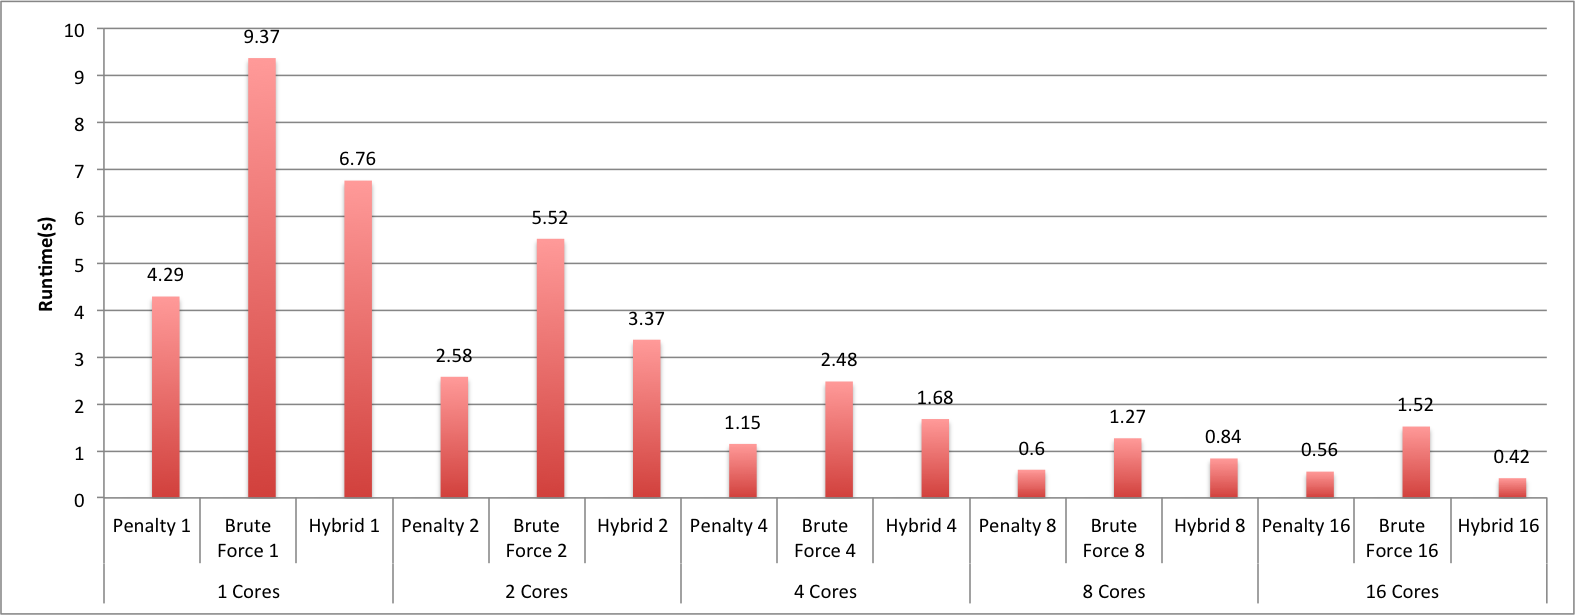
\includegraphics[width=1\textwidth]{experiments/vectorisation/plots/hybrid} \protect\caption{\label{fig17}Hybrid SIMD vs Serial.}

